\section{Problem 1: FFT of Single Tone sinusoidal wave}

\begin{enumerate}
    \item The function generator was set to a sinusoidal wave with a $500$Hz frequency, 2$V_{pp}$ amplitude, and no offset. The measure function was used to verify all the properties of the signal, and a hardcopy was subsequently taken.
          \begin{figure}[H]
              \centering
              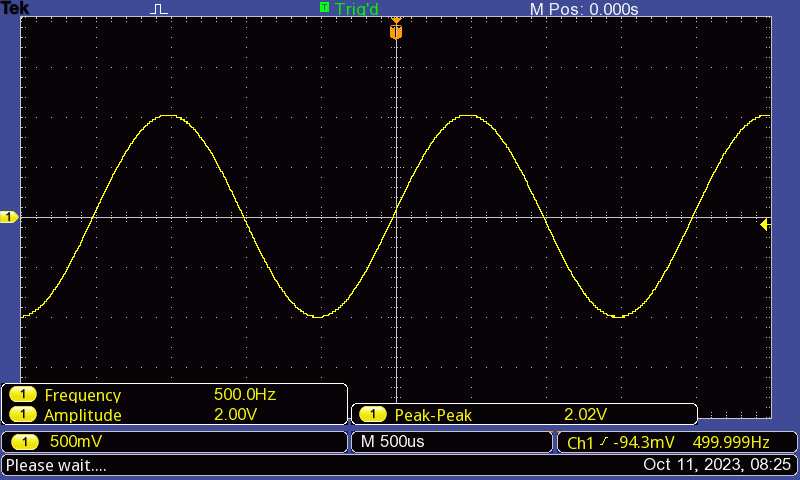
\includegraphics[width=0.8\linewidth]{images/problem1_hardcopy1.png}
              \caption{Hardcopy of the signal}
              \label{fig:problem1_hardcopy1}
          \end{figure}
    \item Afterward, the FFT spectrum was obtained via the spectrum's FFT function. The cursor was used to measure the properties of the spectrum, and then a hardcopy was taken. Furthermore, another hardcopy was taken of the zoomed in spectrum.
          \begin{figure}
              \centering
              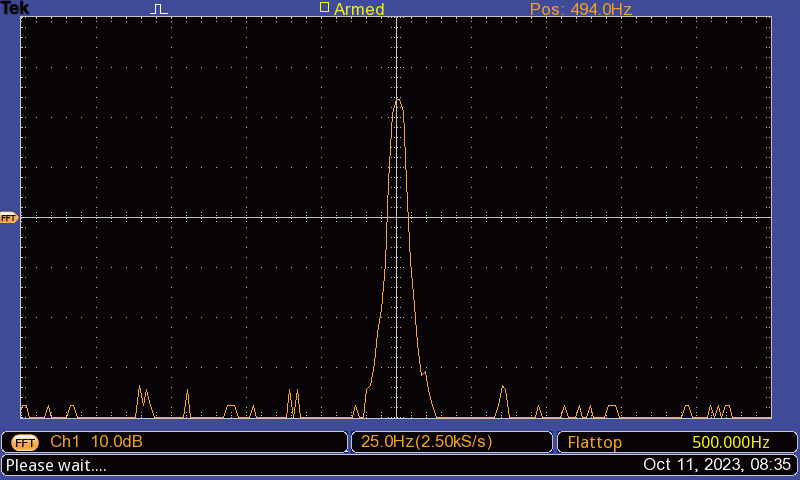
\includegraphics[width=0.5\linewidth]{images/problem1_hardcopy2.png}
              \caption{Hardcopy of the FFT spectrum, showing 494Hz.}
              \label{fig:problem1_hardcopy2}
          \end{figure}
          \begin{figure}[H]
              \centering
              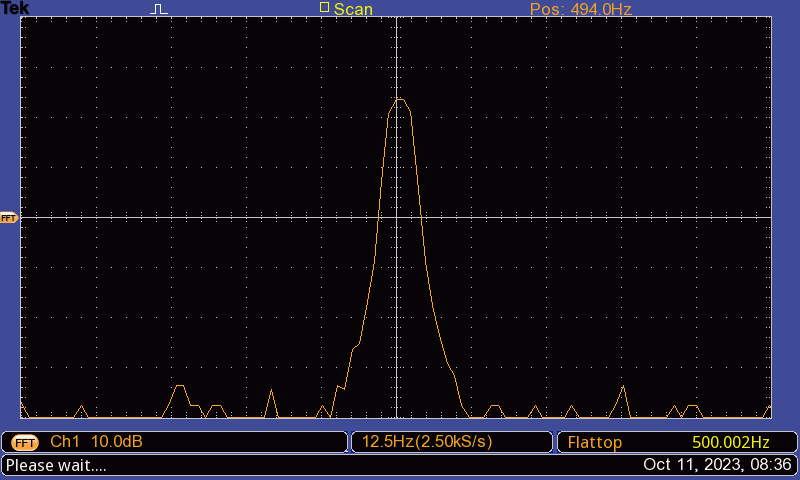
\includegraphics[width=0.5\linewidth]{images/problem1_hardcopy3.png}
              \caption{Hardcopy of the zoomed in FFT spectrum, showing 494Hz.}
              \label{fig:problem1_hardcopy3}
          \end{figure}
          What is immediately noticed, however, is that the position seems to show 494Hz. This is in fact an error of $1\%$, when the usual error should be around $0.1\%$. The reason this error shows up may be due to the miscalibration of the Oscilloscope.
    \item For the sinusoidal wave with a 2KHz frequency(without any offset) to have a 0dB spectrum peak, the $V_{pp}$ was found to be around 2.7$V_{pp}$. A hardcopy of the time-domain signal was taken.
          \begin{figure}[H]
              \centering
              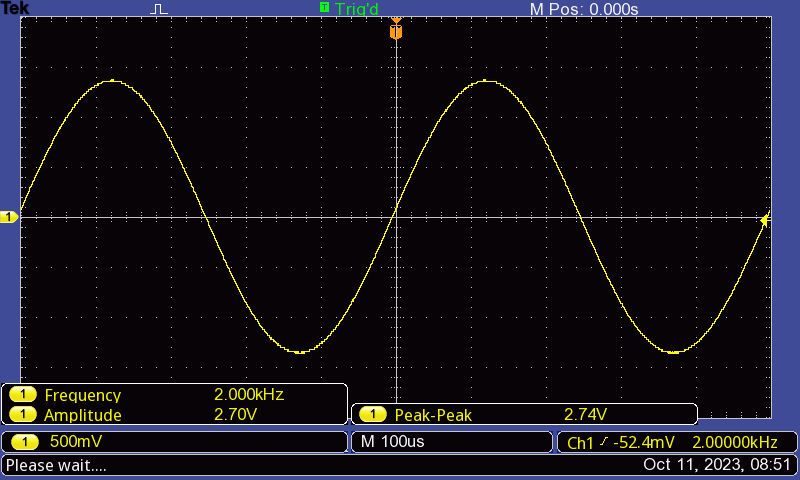
\includegraphics[width=0.75\linewidth]{images/problem1_hardcopy4.png}
              \caption{Hardcopy of the time-domain signal with 0dB spectrum peak.}
              \label{fig:problem1_hardcopy4}
          \end{figure}
          Then, a hardcopy is taken of the frequency spectrum that is obtained by using the FFT function on the oscilloscope.
          \begin{figure}[H]
              \centering
              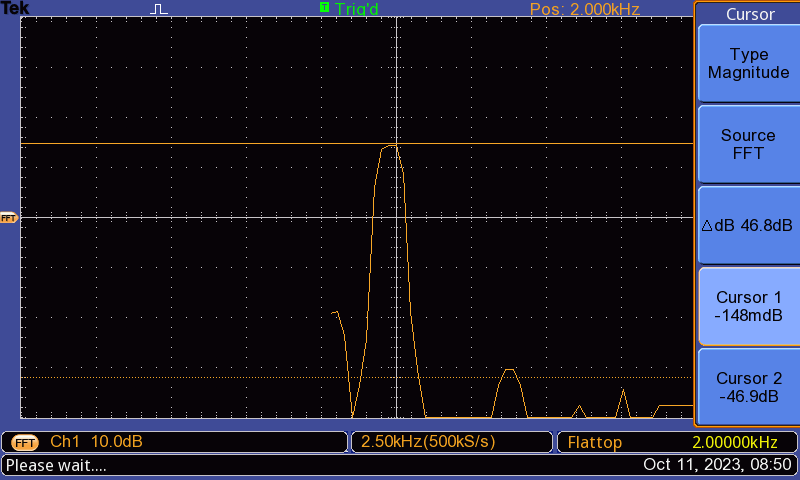
\includegraphics[width=0.75\linewidth]{images/problem1_hardcopy5.png}
              \caption{Hardcopy of the frequency spectrum with 0dB spectrum peak.}
              \label{fig:problem1_hardcopy5}
          \end{figure}
          It is observed that the cursor shows a dB of $-148$mdB which is close to $0$dB. The small error is because of the Oscilloscope's resolution. It also shows the 2KHz frequency.
\end{enumerate}

\section{Problem 2:}